\documentclass[journal,12pt,onecolumn]{IEEEtran}
\usepackage{gvv-book}
\usepackage{gvv}

\begin{document}
\title{2.5.17}
\author{EE25BTECH11054 - S.Harsha Vardhan Reddy}
	\maketitle

\section{Problem 2.5.17}
Find a unit vector perpendicular to both the vectors $\vec{a}$ and $\vec{b}$, where $\vec{a} = \hat{i} - 7\hat{j} + 7\hat{k}$ and $\vec{b} = 3\hat{i} - 2\hat{j} + 2\hat{k}$.

\solution

Given vectors are:
\begin{align}
\vec{a} &= \myvec{1 \\ -7 \\ 7} \\
\vec{b} &= \myvec{3 \\ -2 \\ 2}
\end{align}

A vector perpendicular to both $\vec{a}$ and $\vec{b}$ can be obtained using the cross product $\vec{a} \times \vec{b}$.

\subsection{\textbf{Computing the Cross Product}}

The cross product of $\vec{a}$ and $\vec{b}$ is defined as:
\begin{align}
\vec{a} \times \vec{b} = \mydet{A_{23} & B_{23} \\ A_{31} & B_{31} \\ A_{12} & B_{12}}
\end{align}

where the sub-vectors are defined as:
\begin{align}
A_{ij} = \mydet{a_i \\ a_j}, \quad B_{ij} = \mydet{b_i \\ b_j}
\end{align}

For our given vectors, we identify the components:
\begin{align}
a_1 = 1, \quad a_2 = -7, \quad a_3 = 7 \\
b_1 = 3, \quad b_2 = -2, \quad b_3 = 2
\end{align}

Now, computing the required sub-vectors:
\begin{align}
A_{23} &= \myvec{a_2 \\ a_3} = \myvec{-7 \\ 7} \\
B_{23} &= \myvec{b_2 \\ b_3} = \myvec{-2 \\ 2}
\end{align}

\begin{align}
A_{31} &= \myvec{a_3 \\ a_1} = \myvec{7 \\ 1} \\
B_{31} &= \myvec{b_3 \\ b_1} = \myvec{2 \\ 3}
\end{align}

\begin{align}
A_{12} &= \myvec{a_1 \\ a_2} = \myvec{1 \\ -7} \\
B_{12} &= \myvec{b_1 \\ b_2} = \myvec{3 \\ -2}
\end{align}

For a $2 \times 2$ determinant, we use the formula:
\begin{align}
\mydet{p_1 & q_1 \\ p_2 & q_2} = p_1q_2 - p_2q_1
\end{align}

\subsection{\textbf{Computing Each Component}}

\textbf{First Component:}
\begin{align}
\mydet{A_{23} & B_{23}} &= \mydet{-7 & -2 \\ 7 & 2} \nonumber\\
&= (-7)(2) - (7)(-2) \nonumber\\
&= 0
\end{align}

\textbf{Second Component:}
\begin{align}
\mydet{A_{31} & B_{31}} &= \mydet{7 & 2 \\ 1 & 3} \nonumber\\
&= (7)(3) - (1)(2) \nonumber\\
&= 19
\end{align}

\textbf{Third Component:}
\begin{align}
\mydet{A_{12} & B_{12}} &= \mydet{1 & 3 \\ -7 & -2} \nonumber\\
&= (1)(-2) - (-7)(3) \nonumber\\
&= 19
\end{align}

Therefore, the cross product is:
\begin{align}
\vec{a} \times \vec{b} = \myvec{0 \\ 19 \\ 19}
\end{align}

This vector is perpendicular to both $\vec{a}$ and $\vec{b}$.

\subsection{\textbf{Finding the Unit Vector}}

To obtain a unit vector, we need to divide the cross product vector by its magnitude.

Computing the magnitude of $\vec{a} \times \vec{b}$:
\begin{align}
\norm{\vec{a} \times \vec{b}} &= \sqrt{(0)^2 + (19)^2 + (19)^2} \nonumber\\
&= \sqrt{722} \nonumber\\
&= 19\sqrt{2}
\end{align}

The unit vector in the direction of any vector $\vec{v}$ is obtained by:
\begin{align}
\hat{v} = \frac{\vec{v}}{\norm{\vec{v}}}
\end{align}

Therefore, the required unit vector perpendicular to both $\vec{a}$ and $\vec{b}$ is:
\begin{align}
\hat{n} &= \frac{\vec{a} \times \vec{b}}{\norm{\vec{a} \times \vec{b}}} \nonumber\\
&= \frac{1}{19\sqrt{2}}\myvec{0 \\ 19 \\ 19} \nonumber\\
&= \myvec{0 \\ \frac{19}{19\sqrt{2}} \\ \frac{19}{19\sqrt{2}}} \nonumber\\
&= \myvec{0 \\ \frac{1}{\sqrt{2}} \\ \frac{1}{\sqrt{2}}}
\end{align}

This can be written in component form as:
\begin{align}
\hat{n} = 0\hat{i} + \frac{1}{\sqrt{2}}\hat{j} + \frac{1}{\sqrt{2}}\hat{k}
\end{align}


\begin{align}
\hat{n} = \frac{1}{\sqrt{2}}\brak{\hat{j} + \hat{k}}
\end{align}



\subsection{\textbf{Final Answer}}

The unit vector perpendicular to both $\vec{a} = \hat{i} - 7\hat{j} + 7\hat{k}$ and $\vec{b} = 3\hat{i} - 2\hat{j} + 2\hat{k}$ is:
\begin{align}
\hat{n} = \frac{1}{\sqrt{2}}\brak{\hat{j} + \hat{k}}
\end{align}

\begin{figure}
    \centering
    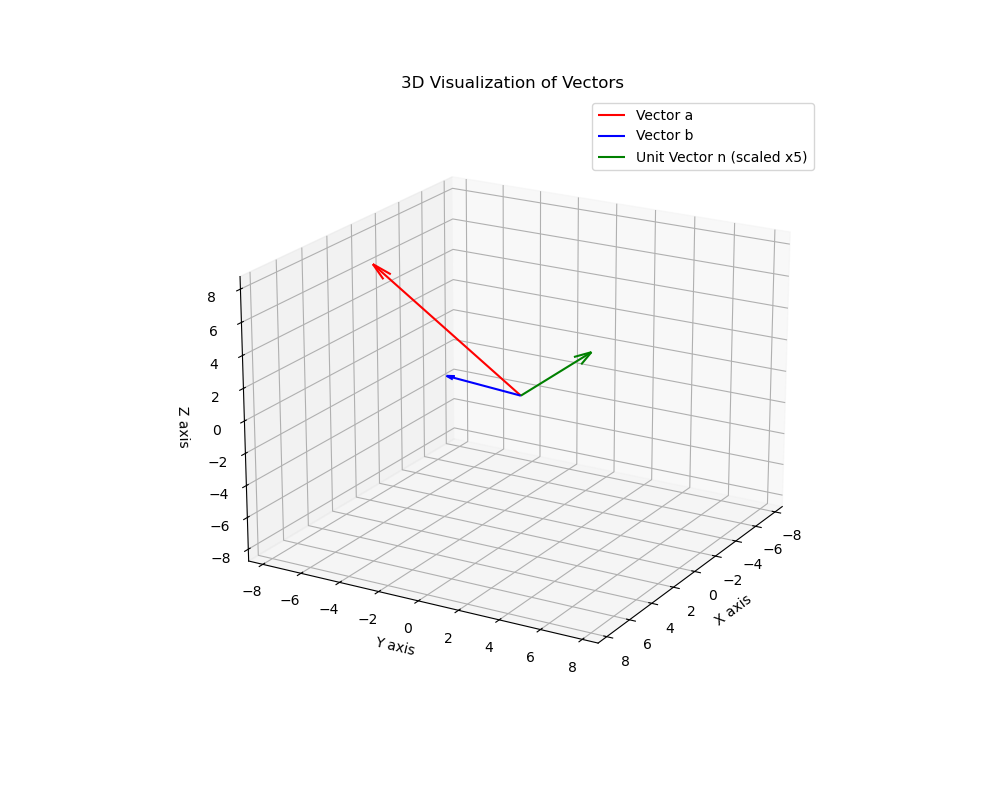
\includegraphics[width=1.0\columnwidth]{figs/2.5.17 .png}
    \caption{}
    \label{fig:placeholder}
\end{figure}

\end{document}